\chapter{Estrutura de Banco de Dados}
\label{c:estrutura_de_banco_de_dados}
% ---
Descrito o Sistema de infraestrutura da rede, é necessário que os dados dos medidores sejam armazenados para possibilitar consultas futuras. Para isso foi desenvolvida uma estrutura de dados onde pode-se armazenar os dados dos medidores e de suas respectivas medições.Além disso, outro requisito do sistema era que os dados referente às unidades consumidoras pudessem ser armazenados, bem como os dados das suas faturas geradas pela concessionária de energia, com os valores oficiais de medição e cobrança.

Abaixo pode-se observar o layout do modelo de dados com as entidades principais do projeto e seus atributos, bem como suas relações.

\begin{figure}[H]
    \centering
    \caption{Diagrama do Modelo de Dados SIDE}
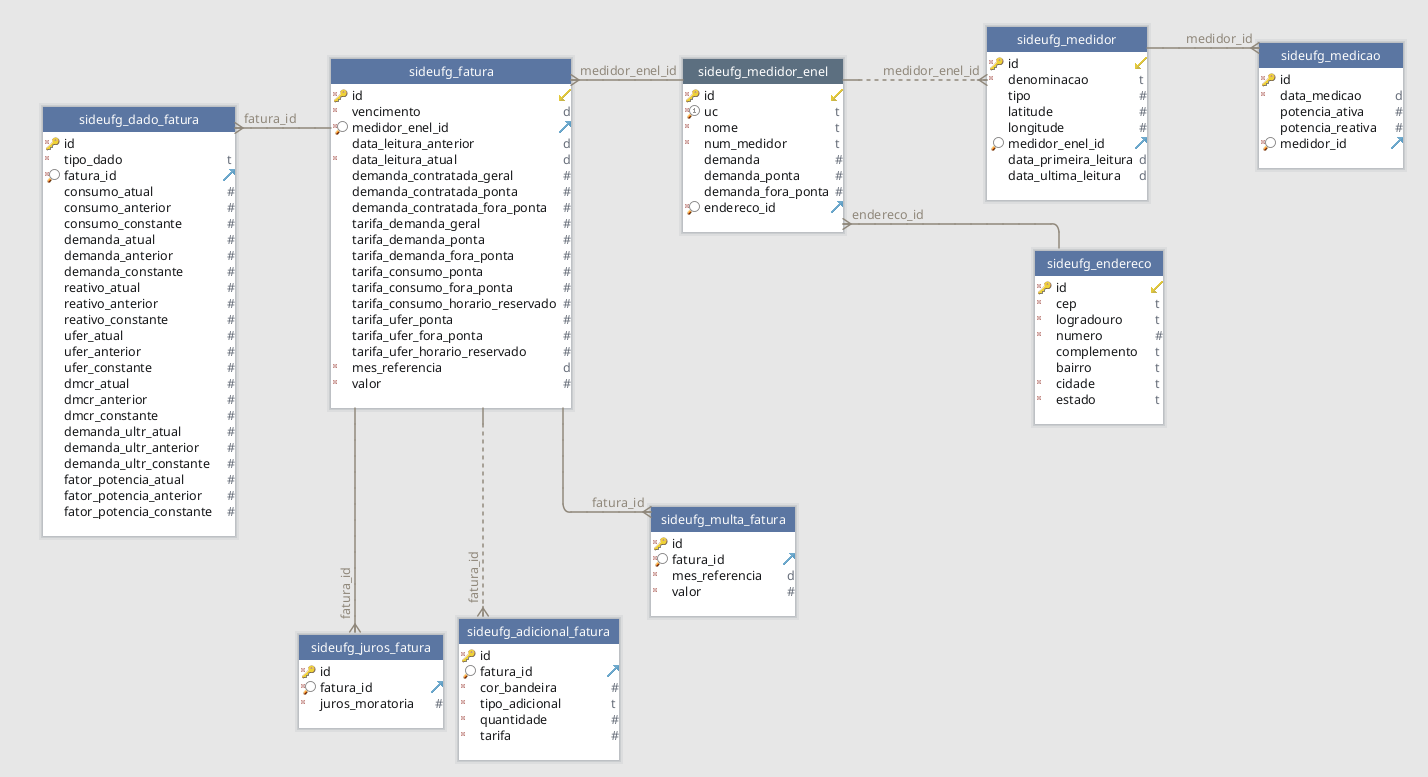
\includegraphics[width=\linewidth]{imagens/modelo-de-dados-side.png}
    \caption*{Fonte: Próprio Autor}
    \label{fig:diagrama-modelo-dados}
\end{figure}

A modelagem da figura \ref{fig:diagrama-modelo-dados}, pode ser visualizada através de um modelo online criado no \textit{software DbSchema}, acessível através do link disponível no apêndice \ref{a:PFC1}.


Devido ao uso de um \textit{framework} para desenvolvimento ágil não se fez necessário preocupar-se com as estruturas de dados referentes a acessos dos usuários, cadastro, definição de papéis, preferências de acesso, bem como criação de versionamento para a criação de um histórico de alteração dos dados do banco. Na figura acima foram omitidas todas as tabelas criadas pelo \textit{framework} Cuba, com a finalidade de focar o modelo no problema específico da aplicação. Toda a documentação referente ao \textit{framework} pode ser encontrada em seu \textit{site} oficial.

\section{Tabela de Medidores da Concessionária}

A tabela onde é feito o cadastro dos Medidores da Concessionária é a tabela \textbf{sideufg\_medidor\_enel} onde os registros são identificados através do campo \textbf{id} do tipo UUID.

Nesta tabela são armazenados os seguintes campos:

\begin{itemize}
    \item \textbf{uc} - Campo obrigatório do tipo \textit{varchar(20)} para armazenar a número da Unidade Consumidora;
    \item \textbf{nome} - Campo obrigatório do tipo \textit{varchar(100)} para armazenar uma denominação para o Medidor;
    \item \textbf{num\_medidor} - Campo obrigatório do tipo \textit{varchar(20)} para armazenar o número do medidor daquele ponto de medição;
    \item \textbf{demanda} - Campo do tipo \textit{integer} para armazenar a demanda contratada para aquela Unidade Consumidora quando a mesma não possui contrato específico por período de medição;
    \item \textbf{demanda\_ponta} - Campo do tipo \textit{integer} para armazenar a demanda contratada para aquela Unidade Consumidora no período de ponta;
    \item \textbf{demanda\_fora\_ponta} - Campo do tipo \textit{integer} para armazenar a demanda contratada para aquela Unidade Consumidora no período fora de ponta;
    \item \textbf{endereco\_id} - Campo do tipo UUID com uma chave estrangeira para armazenar a chave primária do endereço relacionado àquele medidor;
\end{itemize}

\section{Tabela de Medidores da UFG}

A tabela onde é feito o cadastro dos Medidores da CCK é a tabela \textbf{sideufg\_medidor} onde os registros são identificados através do campo \textbf{id} do tipo UUID.
\newpage
Nesta tabela são armazenados os seguintes campos:

\begin{itemize}
    \item \textbf{denominacao} - Campo obrigatório do tipo varchar(255) para armazenar uma denominação para o Medidor;
    \item \textbf{tipo} - Campo do tipo \textit{integer} para armazenar o tipo do medidor podendo ser:
    \subitem 10 - CCK 4400ME;
    \subitem 20 - CCK 6700E;
    \item \textbf{latitude} - Campo do tipo \textit{float8} para armazenar a latitude do medidor para georreferenciamento;
    \item \textbf{longitude} - Campo do tipo \textit{float8} para armazenar a longitude do medidor para georreferenciamento;
    \item \textbf{medidor\_enel\_id} - Campo do tipo UUID com uma chave estrangeira para armazenar a chave primária da unidade consumidora relacionada àquele medidor;
    \item \textbf{data\_primeira\_leitura} - Campo do tipo \textit{timestamp} para armazenar o momento a partir do qual o medidor começou a enviar dados para a base;
    \item \textbf{data\_ultima\_leitura} - Campo do tipo \textit{timestamp} para armazenar o momento da última leitura que o \textit{SIDE Synchronizer} obteve do medidor;
    
\end{itemize}

\section{Tabela de Medições}

A tabela onde é feito o cadastro das medições feitas pelos dispositivos da CCK é a tabela \textbf{sideufg\_medicao} onde os registros são identificados através do campo \textbf{id} do tipo UUID.

Nesta tabela são armazenados os seguintes campos:

\begin{itemize}
    \item \textbf{data\_medicao} - Campo do tipo \textit{timestamp} para armazenar o momento no qual o medidor fez o registro da medição em sua memória de massa;
    \item \textbf{potencia\_ativa} - Campo do tipo \textit{float8} para armazenar o valor de potencia ativa medido;
    \item \textbf{potencia\_reativa} - Campo do tipo \textit{float8} para armazenar o valor de potencia reativa medido;
    \item \textbf{medidor\_id} - Campo do tipo UUID com uma chave estrangeira para armazenar a chave primária do medidor CCK relacionado àquela medição;
\end{itemize}

\section{Tabela de Endereços}

A tabela onde é feito o cadastro dos Endereços das Unidades Consumidoras da UFG é a tabela \textbf{sideufg\_endereco} onde os registros são identificados através do campo \textbf{id} do tipo UUID.

Nesta tabela são armazenados os seguintes campos:

\begin{itemize}
    \item \textbf{cep} - Campo obrigatório do tipo \textit{varchar(8)} para armazenar o CEP do endereço;
    \item \textbf{logradouro} - Campo obrigatório do tipo \textit{varchar(100)} para armazenar o logradouro do endereço;
    \item \textbf{numero} - Campo obrigatório do tipo \textit{integer} para armazenar o número do endereço;
    \item \textbf{complemento} - Campo do tipo \textit{varchar(100)} para armazenar o complemento do endereço;
    \item \textbf{bairro} - Campo do tipo \textit{varchar(100)} para armazenar o bairro do endereço;
    \item \textbf{cidade} - Campo obrigatório do tipo \textit{varchar(100)} para armazenar a cidade do endereço;
    \item \textbf{estado} - Campo obrigatório do tipo \textit{varchar(50)} para armazenar a sigla do estado do endereço, onde a busca pela sigla ocorre através de uma seleção no cadastro através de um \textit{enumeration};
    
\end{itemize}

\section{Estrutura de Dados para Armazenamento das Faturas}

As faturas energéticas das unidades consumidoras possuem um grande volume de dados que são importantes para as análises econômicas, quantitativas e qualitativas do consumo das edificações da Universidade. Desde os dados financeiros como valor, tarifas individuais, adicionais tarifários, contratos de demanda, até dados referentes ao consumo propriamente dito com as leituras nos horários específicos de ponta, fora de ponta e horário reservado.

Para a modelagem dessa estrutura de dados foi pensado em uma divisão em cinco tabelas, sendo uma tabela principal contendo os principais dados da fatura, e quatro auxiliares contendo desde dados esporádicos como multa e juros até dados repetitivos como as várias leituras de demanda, consumo, UFER, entre outros na fatura.

\newpage

As tabelas criadas referente ao armazenamento das faturas estão listadas abaixo e serão detalhadas nas sub-sessões \ref{sub:tabela-fatura}, \ref{sub:tabela-dado-fatura}, \ref{sub:tabela-adicional-fatura}, \ref{sub:tabela-multa-fatura} e \ref{sub:tabela-juros-fatura}:

\begin{itemize}
    \item sideufg\_fatura;
    \item sideufg\_dado\_fatura;
    \item sideufg\_adicional\_fatura;
    \item sideufg\_multa\_fatura;
    \item sideufg\_juros\_fatura;
\end{itemize}

\subsection{Tabela de Faturas}
\label{sub:tabela-fatura}

A tabela onde é feito o cadastro das faturas de cada Unidade Consumidora é a tabela \textbf{sideufg\_fatura} onde os registros são identificados através do campo \textbf{id} do tipo UUID.

Nesta tabela são armazenados os seguintes campos:

\begin{itemize}
    \item \textbf{vencimento} - Campo obrigatório do tipo \textit{date} para armazenar a data de vencimento da fatura;
    \item \textbf{medidor\_enel\_id} - Campo obrigatório do tipo UUID com uma chave estrangeira para armazenar a chave primária da unidade consumidora relacionada àquela fatura;
    \item \textbf{data\_leitura\_anterior} - Campo do tipo \textit{date} para armazenar a data da leitura da fatura anterior;
    \item \textbf{data\_leitura\_atual} - Campo obrigatório do tipo \textit{date} para armazenar a data da leitura atual da fatura;
    \item \textbf{demanda\_contratada\_geral} - Campo do tipo \textit{integer} para armazenar a demanda contratada naquele mês para aquela Unidade Consumidora quando a mesma não possui contrato específico por período de medição;
    \item \textbf{demanda\_contratada\_ponta} - Campo do tipo \textit{integer} para armazenar a demanda contratada naquele mês para aquela Unidade Consumidora no período de ponta;
    \item \textbf{demanda\_contratada\_fora\_ponta} - Campo do tipo \textit{integer} para armazenar a demanda contratada naquele mês para aquela Unidade Consumidora no período fora de ponta;
    \item \textbf{tarifa\_demanda\_geral} - Campo do tipo \textit{big decimal (19,6)} para armazenar a tarifa da demanda geral naquele mês;
    \item \textbf{tarifa\_demanda\_ponta} - Campo do tipo \textit{big decimal (19,6)} para armazenar a tarifa da demanda no horário de ponta naquele mês;
    \item \textbf{tarifa\_demanda\_fora\_ponta} - Campo do tipo \textit{big decimal (19,6)} para armazenar a tarifa da demanda no horário fora de ponta naquele mês;
    \item \textbf{tarifa\_consumo\_ponta} - Campo do tipo \textit{big decimal (19,6)} para armazenar a tarifa do consumo no horário de ponta naquele mês;
    \item \textbf{tarifa\_consumo\_fora\_ponta} - Campo do tipo \textit{big decimal (19,6)} para armazenar a tarifa do consumo no horário fora de ponta naquele mês;
    \item \textbf{tarifa\_consumo\_horario\_reservado} - Campo do tipo \textit{big decimal (19,6)} para armazenar a tarifa do consumo no horário reservado naquele mês;
    \item \textbf{tarifa\_ufer\_ponta} - Campo do tipo \textit{big decimal (19,6)} para armazenar a tarifa da UFER no horário de ponta naquele mês;
    \item \textbf{tarifa\_ufer\_fora\_ponta} - Campo do tipo \textit{big decimal (19,6)} para armazenar a tarifa da UFER no horário fora de ponta naquele mês;
    \item \textbf{tarifa\_ufer\_horario\_reservado} - Campo do tipo \textit{big decimal (19,6)} para armazenar a tarifa da UFER no horário reservado naquele mês;
    \item \textbf{mes\_referencia} - Campo obrigatório do tipo \textit{date} para armazenar o mês de referência da fatura;
    \item \textbf{valor} - Campo obrigatório do tipo \textit{big decimal (19,2)} para armazenar o valor final da fatura;
\end{itemize}

\subsection{Tabela dos Dados da Fatura}
\label{sub:tabela-dado-fatura}
A tabela onde é feito o cadastro dos dados específicos da fatura adquiridos pela interpretação da tabela da segunda página das faturas como a do exemplo da imagem abaixo é a tabela  \textbf{sideufg\_dado\_fatura} onde os registros são identificados através do campo \textbf{id} do tipo UUID.

\begin{figure}[H]
    \centering
    \caption{Modelo de Tabela de Dados Específicos da Fatura}
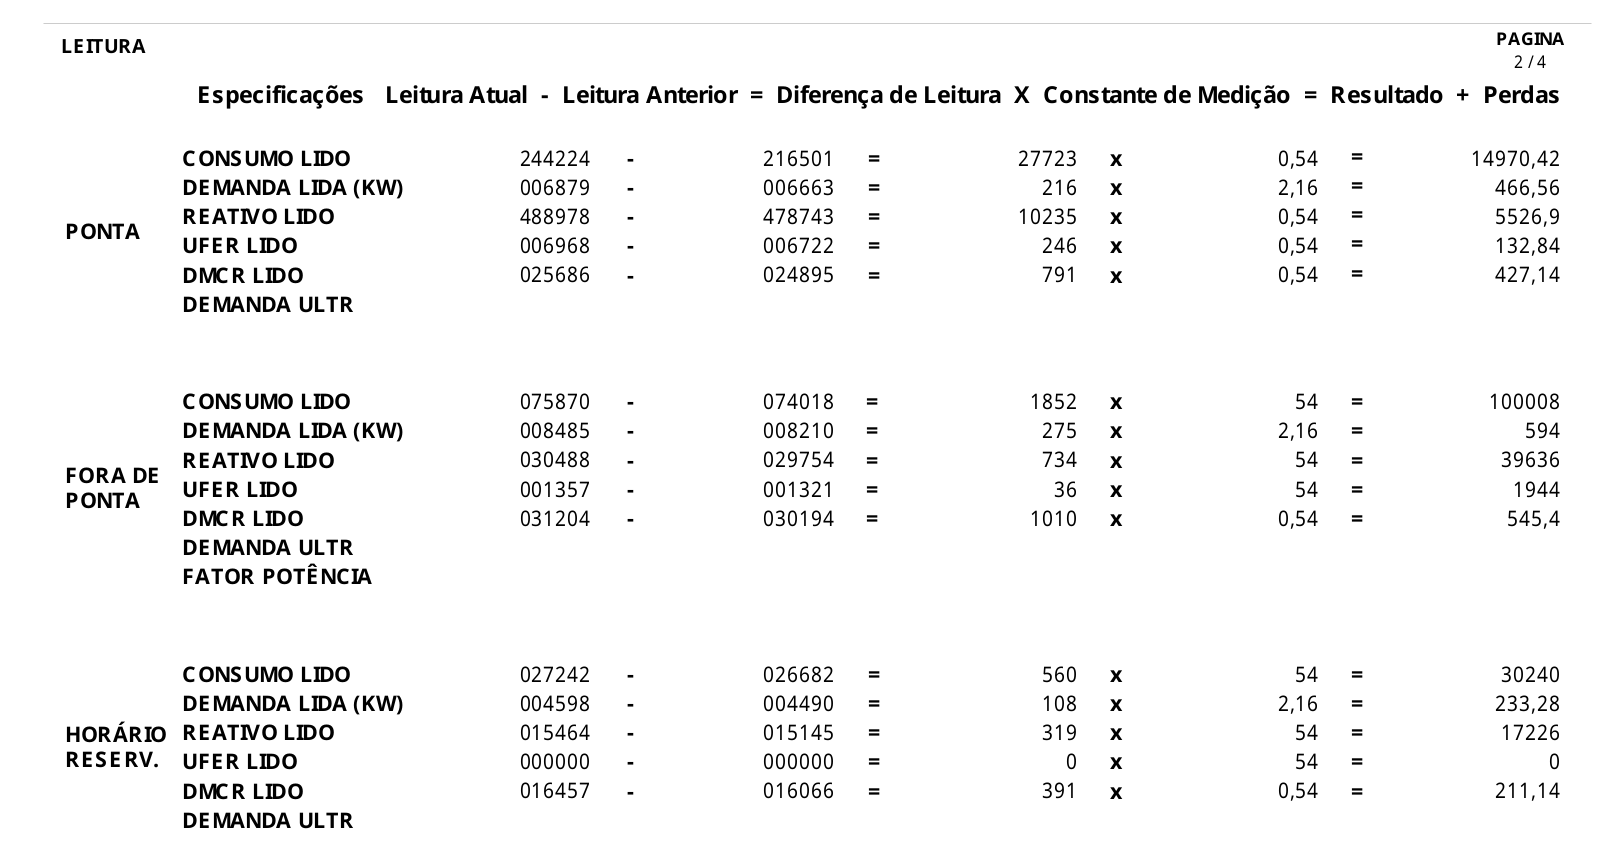
\includegraphics[width=0.8\linewidth]{imagens/modelo-tabela-dados-fatura.png}
    \caption*{Fonte: Próprio Autor}
    \label{fig:modelo-tabela-dados-fatura}
\end{figure}

Nesta tabela são armazenados os seguintes campos:

\begin{itemize}
    \item \textbf{tipo\_dado} - Campo obrigatório do tipo \textit{varchar(50)} para armazenar o tipo da leitura, podendo ser:
    \subitem P - Ponta;
    \subitem F - Fora de Ponta;
    \subitem H - Horário Reservado;
    \item \textbf{fatura\_id} - Campo obrigatório do tipo UUID com uma chave estrangeira para armazenar a chave primária da fatura relacionada àquele dado;
    
    \item \textbf{consumo\_atual} - Campo do tipo \textit{integer} para armazenar a leitura atual de consumo do dado da fatura;
    \item \textbf{consumo\_anterior} - Campo do tipo \textit{integer} para armazenar a leitura anterior de consumo do dado da fatura;
    \item \textbf{consumo\_constante} - Campo do tipo \textit{float8} para armazenar a constante de medição do consumo do dado da fatura;
    
    \item \textbf{demanda\_atual} - Campo do tipo \textit{integer} para armazenar a leitura atual de demanda do dado da fatura;
    \item \textbf{demanda\_anterior} - Campo do tipo \textit{integer} para armazenar a leitura anterior de demanda do dado da fatura;
    \item \textbf{demanda\_constante} - Campo do tipo \textit{float8} para armazenar a constante de medição da demanda do dado da fatura;
    
    \item \textbf{reativo\_atual} - Campo do tipo \textit{integer} para armazenar a leitura atual de reativo do dado da fatura;
    \item \textbf{reativo\_anterior} - Campo do tipo \textit{integer} para armazenar a leitura anterior de reativo do dado da fatura;
    \item \textbf{reativo\_constante} - Campo do tipo \textit{float8} para armazenar a constante de medição do reativo do dado da fatura;
    
    \item \textbf{ufer\_atual} - Campo do tipo \textit{integer} para armazenar a leitura atual de consumo de energia reativa do dado da fatura;
    \item \textbf{ufer\_anterior} - Campo do tipo \textit{integer} para armazenar a leitura anterior de consumo de energia reativa do dado da fatura;
    \item \textbf{ufer\_constante} - Campo do tipo \textit{float8} para armazenar a constante de medição do consumo de energia reativa do dado da fatura;
    
    \item \textbf{dmcr\_atual} - Campo do tipo \textit{integer} para armazenar a leitura atual de demanda máxima corrigida do dado da fatura;
    \item \textbf{dmcr\_anterior} - Campo do tipo \textit{integer} para armazenar a leitura anterior de demanda máxima corrigida do dado da fatura;
    \item \textbf{dmcr\_constante} - Campo do tipo \textit{float8} para armazenar a constante de medição da demanda máxima corrigida  do dado da fatura;
    
    \item \textbf{demanda\_ultr\_atual} - Campo do tipo \textit{integer} para armazenar a leitura atual de demanda ultrapassada do dado da fatura;
    \item \textbf{demanda\_ultr\_anterior} - Campo do tipo \textit{integer} para armazenar a leitura anterior de demanda ultrapassada do dado da fatura;
    \item \textbf{demanda\_ultr\_constante} - Campo do tipo \textit{float8} para armazenar a constante de medição da demanda ultrapassada do dado da fatura;
    
    \item \textbf{fator\_potencia\_atual} - Campo do tipo \textit{integer} para armazenar a leitura atual de fator de potência do dado da fatura;
    \item \textbf{fator\_potencia\_anterior} - Campo do tipo \textit{integer} para armazenar a leitura anterior de fator de potência do dado da fatura;
    \item \textbf{fator\_potencia\_constante} - Campo do tipo \textit{float8} para armazenar a constante de fator de potência do dado da fatura;
    
    
\end{itemize}

\subsection{Tabela dos Adicionais Tarifários da Fatura}
\label{sub:tabela-adicional-fatura}

A tabela onde é feito o cadastro dos adicionais tarifários de bandeira de cada fatura é a tabela \textbf{sideufg\_adicional\_fatura} onde os registros são identificados através do campo \textbf{id} do tipo UUID.

Nesta tabela são armazenados os seguintes campos:

\begin{itemize}
    \item \textbf{fatura\_id} - Campo obrigatório do tipo UUID com uma chave estrangeira para armazenar a chave primária da fatura relacionada àquele adicional;
    \item \textbf{cor\_bandeira} - Campo obrigatório do tipo \textit{integer} para armazenar a cor da bandeira do adicional daquele mês para aquela fatura, podendo ser:
    \subitem 1 - Verde;
    \subitem 2 - Amarela;
    \subitem 3 - Vermelha;
    \item \textbf{tipo\_adicional} - Campo obrigatório do tipo \textit{varchar(50)} para armazenar o tipo do adicional tarifário, podendo ser:
    \subitem P - Ponta;
    \subitem F - Fora de Ponta;
    \subitem H - Horário Reservado;
    \item \textbf{quantidade} - Campo obrigatório do tipo \textit{big decimal (13,2)} para armazenar a quantidade do adicional a ser cobrado naquele mês naquela fatura;
    \item \textbf{tarifa} - Campo obrigatório do tipo \textit{big decimal (19,6)} para armazenar a tarifa do adicional a ser cobrado naquele mês naquela fatura;
\end{itemize}

\subsection{Tabela das Multas da Fatura}
\label{sub:tabela-multa-fatura}

A tabela onde é feito o cadastro das multas aplicadas à cada fatura é a tabela \textbf{sideufg\_multa\_fatura} onde os registros são identificados através do campo \textbf{id} do tipo UUID.

Nesta tabela são armazenados os seguintes campos:

\begin{itemize}
    \item \textbf{fatura\_id} - Campo obrigatório do tipo UUID com uma chave estrangeira para armazenar a chave primária da fatura relacionada àquela multa;
    \item \textbf{mes\_referencia} - Campo obrigatório do tipo \textit{date} para armazenar o mês de referência da multa da fatura;
    \item \textbf{valor} - Campo obrigatório do tipo \textit{big decimal (13,2)} para armazenar o valor da multa da fatura;
\end{itemize}

\subsection{Tabela dos Juros da Fatura}
\label{sub:tabela-juros-fatura}

A tabela onde é feito o cadastro dos juros monetários aplicados à cada fatura é a tabela \textbf{sideufg\_juros\_fatura} onde os registros são identificados através do campo \textbf{id} do tipo UUID.

Nesta tabela são armazenados os seguintes campos:

\begin{itemize}
    \item \textbf{fatura\_id} - Campo obrigatório do tipo UUID com uma chave estrangeira para armazenar a chave primária da fatura relacionada àquele juros;
    \item \textbf{juros\_moratoria} - Campo obrigatório do tipo \textit{big decimal (13,2)} para armazenar o valor dos juros da fatura;
\end{itemize}